% !TEX TS-program = lualatex
%\documentclass[handout]{beamer}
\documentclass{beamer}
\input{../common/misomva}
\begin{document}
% Topic-specific title slide
\newcommand{\topictitle}{Random Graph Models}
\newcommand{\topicsubtitle}{Erdős–Rényi, Barabási–Albert, and Stochastic Blocks}
\newcommand{\misoclasstinytitleslide}{Partially based on material by:  Andreas Krause, \\[-1em] Branislav Kveton, Michael Kearns}

\MakeTopicSlide

\begin{frame}
\frametitle{The in-between option: random graph models}
\begin{columns}
\begin{column}{.33\textwidth}
\textbf{Erd\H os-R\' enyi}
{\small independent edges} 
\bigskip
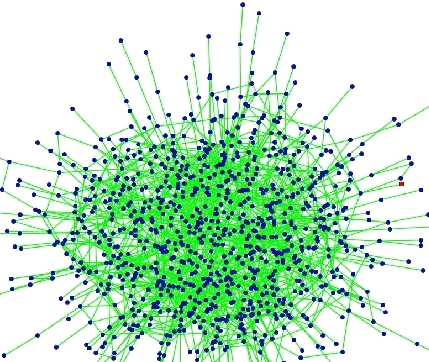
\includegraphics[width=0.9\textwidth]{../img/er_transparent}\\
\end{column}
\pause
\begin{column}{.33\textwidth}
\textbf{Barab\'asi-Albert}
\bigskip
{\small preferential attachment}  
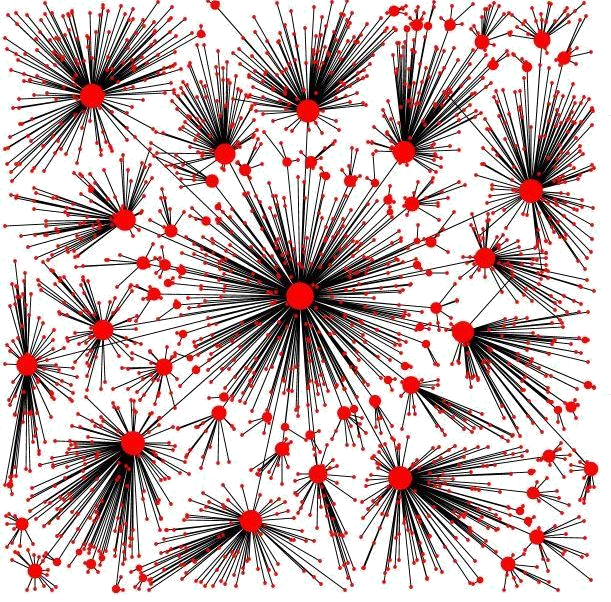
\includegraphics[width=0.8\textwidth]{../img/bamodel_transparent}\\
\end{column}
\pause
\begin{column}{.35\textwidth}
\textbf{Stochastic Blocks}
{\small modeling communities}  
\bigskip
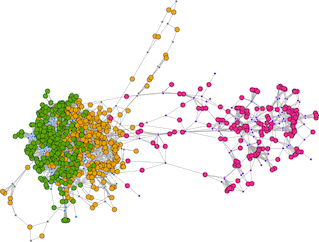
\includegraphics[width=\textwidth]{../img/sbm_transparent}\\
\end{column}
\end{columns}
\bigskip
\pause Watts-Strogatz, Chung-Lu, Fiedler, \dots.

\end{frame}

\usebackgroundtemplate{%
\tikz\node {%
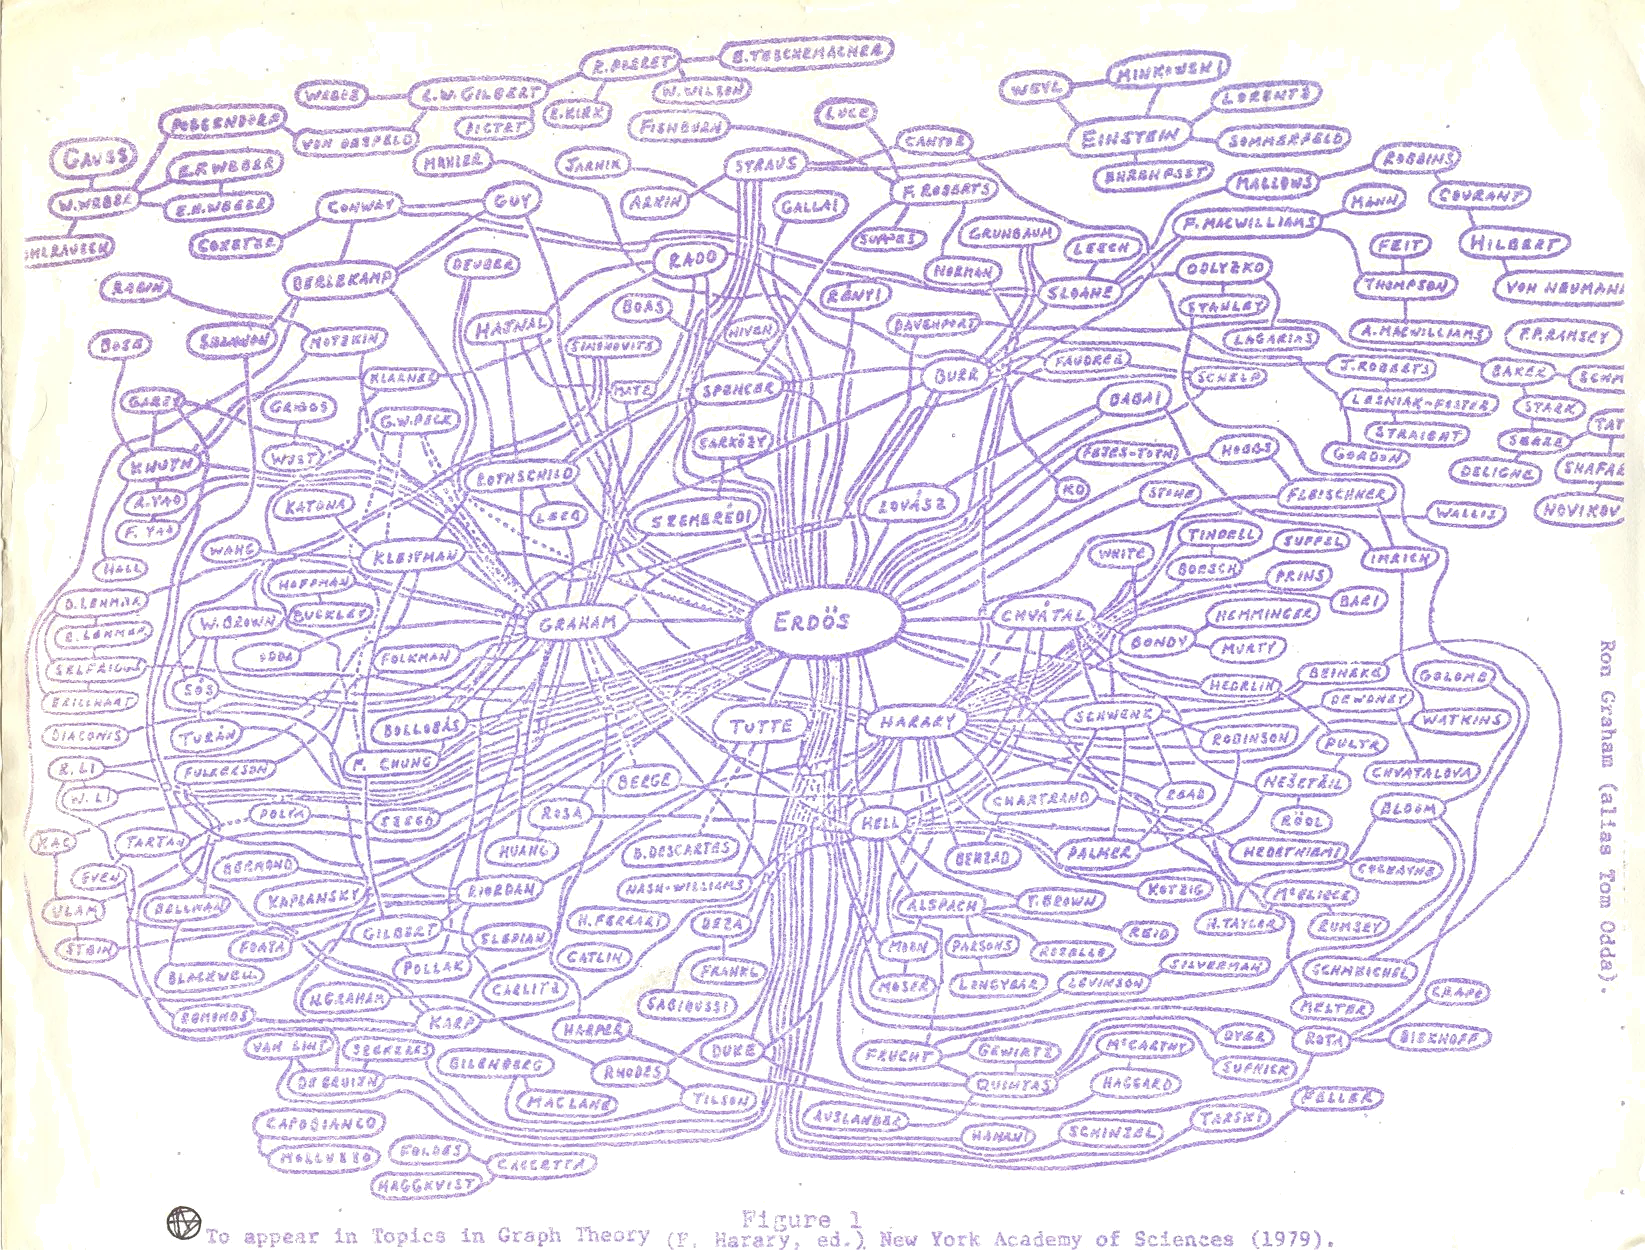
\includegraphics[width=\paperwidth]{../img/cgraph}
};}


\begin{frame}
% 
\includegraphics[width=\paperwidth]{img/cgraph}
\end{frame}

\usebackgroundtemplate{%
\tikz\node[opacity=0.10] {%
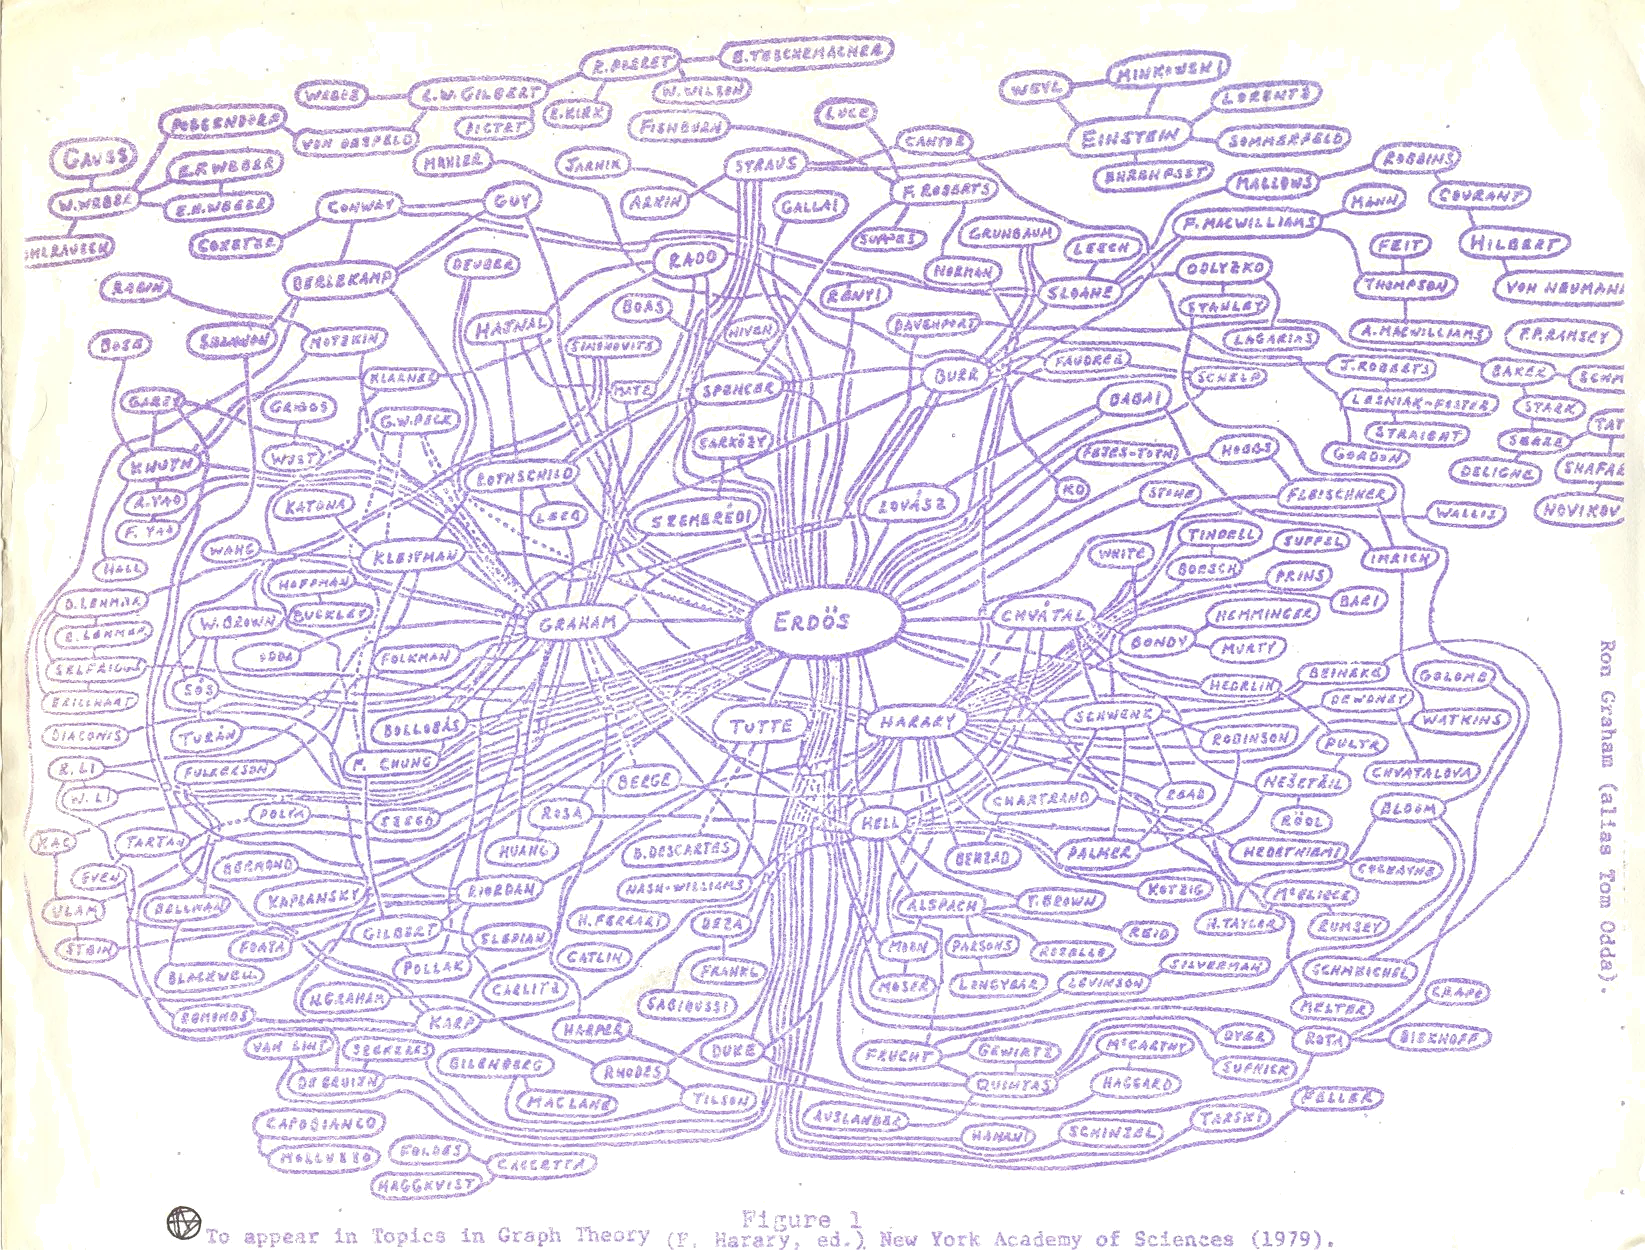
\includegraphics[width=\paperwidth]{../img/cgraph}
};}

\begin{frame}
\frametitle{Erd\H os number project}
\begin{itemize}[<+-| alert@+>]\addtolength{\itemsep}{0.5\baselineskip}
\item \url{http://www.oakland.edu/enp/} \emphcol{try it!}
\item an example of a real-world graph
\item 401 000 authors, 676 000 edges ($\ll 401000^2 \to$ sparse)
\item average degree 3.36
\item average distance for the largest component: 7.64 
\item 6 degrees of separation [Travers \& Milgram, 1967]
\item heavy tail
\end{itemize}

\end{frame}

\usebackgroundtemplate{}


\MakeLastSlide
\end{document}
